\chapter{Literature}\label{Lit:Literature}

\section{Solar Voltaic Cells}

\label{sec:Intro}
A solar voltaic cell is able to convert solar energy into electrical energy by means of the photo voltaic effect. The photo voltaic effect occurs when a N-type and P-Type material are connected .This means that light generated carriers are swept across a p-n barrier, electrons move to the n-side and holes move to the p-side. The barrier prevents the holes and electrons from returning to their original locations and this causes a net electric charge \cite{PVEducation}. 


\label{sec:OC}
The open circuit voltage of a solar cell is the maximum voltage when no current is flowing \cite{PVeduOC}. The solar module in question has a rated open circuit voltage of 22.31V. This solar module has 36 cells in series which means the voltage of each cell sums up to 22.31V. This implies that each solar cell at its maximum will have a voltage of $\frac{22.32}{36}=0.62V$. The open circuit voltage in general is dependant on factors such as temperature. An increase in temperature will lead to a lower $V_{OC}$\cite{PVeduOC}.

\label{sec:SC}
Short circuit current is when the terminals of the solar cell/module is shorted and the voltage across the terminals is 0V. The short circuit current is dependant on the spectrum of the light shining on the PV module, something called the collection probability, the optical properties (absorption and reflection) and the number of photons that the panel is exposed to which can be split into the area of the cell/module and the intensity of the light. The collection probability of the solar cell is dependant on the minority carrier lifetime . This means the average time it takes for the excess minority carrier to recombine\cite{Frei}.


\label{sec:MPPT}
From figure \ref{fig:mppt} it can be seen that there are two points at which the lines have definite changes.The "knee" of the I-V curve and the "elbow" of the PV curve. 
\begin{wrapfigure}{l}{0.4\textwidth}
\centering
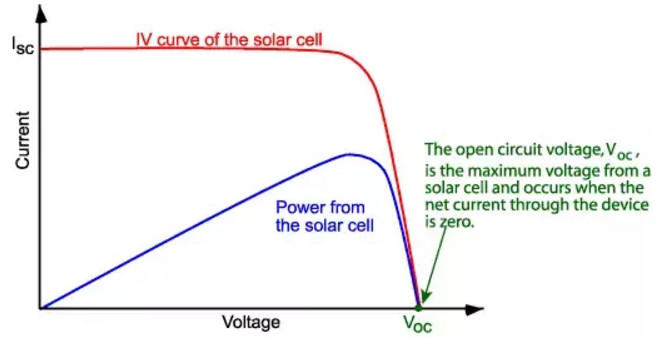
\includegraphics[width=0.36\textwidth]{Figures/MPPT.png}
\caption{Maximum power point tracking \cite{MPPT}}
\label{fig:mppt}
\end{wrapfigure}
The voltage at which the peak of the PV curve occurs is the voltage at which the maximum power is achieved. When external factors change such as temperature, light intensity and spectrum of the light, it causes the I-V and P-V curves to change \cite{vidmppt}. Under standard conditions the MPP of the solar panel in question occurs at 18.21V and 0.28A. To calculate the efficiency of the solar panel you take the radiance of the light shining on the module and multiply it by the area of the module. This is the ideal maximum power for that light. To get efficiency divide the previous answer by the power output. In general solar panels have an efficiency of 20\%\cite{eff}. 



\label{sec:STC}
The Standard Test conditions used to test the SLP005-12 solar panel is a light that emits 1000W per square meter and the light used had an AM of 1.5. The tests were completed at 25$^{\circ}$C.The Standard Testing conditions are parameter that all solar panel producers use to define the performance of their solar equipment.





\begin{table}[!htb]
        \centering
        \footnotesize
        \caption{Solar Panel Measurements}
         \begin{tabular}{lrrrr}
          \toprule
             & $V_{O.C}$ & $I_{S.C}$ & $V_{pmax}$ \\
             &  [V]  & [mA] & [V]\\
          \midrule
          Theroretical per cell & 0.6      & 340 & 0.472 \\
          Datasheet  per module &  21.6      & 340 & 17 \\
          Measured dark       & 1.1 & 0 \\
          Measured upside-down  19.19      & 7.8 & 1.0 \\
          Measured oblique       & 19.7 & 33 \\
          Measured facing        & 22.66 & 178.3 \\
          \bottomrule
        \end{tabular}
     \label{tab:PVresults}
\end{table}

%%%%%%%%%%%%%%%%%%%%%%%%%%%%%%%%%%%%%%%%%%%%%%%%%%%%%%%%%%%%%%%%%%%%%%%%%%%%%%%%%%%
\section{Lead Acid Battery}
\label{sec:Bat Intro}


\label{sec:batchar}
The battery capacity of a Lead acid battery can not be used from 100\% to 0\% but instead the battery data sheet discharges to a minimum of 1.8V per cell (5.4V). The battery in our use case is rated for 4.0Ah@20hr-rate to 1.80V which means that it was able to discharge for 20hr with a load of 0.2A until the voltage of each cell reaches 1.8V. The capacity of a lead acid battery is affected by a number of external factors such as temperature. Higher temperatures will increase capacity at the cost of accelerating ageing of the battery and lower temperatures will decrease the battery capacity  \cite{PVEducation}.

 Batteries also have an internal resistance, in our case 45m\textohm. This internal resistance will have the effect of heating the battery up. The internal resistance of the battery increases with lower temperatures and decreases with higher temperatures[2]. The battery used in E344 has a self discharge of 3\% per month at room temperature. The internal resistance can also cause a voltage drop \cite{BatteryUniversity} at the terminals when the battery is connected to a load, this can be seen in figure \ref{fig:discharge}.


\label{sec:BatteryCharging}
\begin{wrapfigure}{l}{0.4\textwidth}
\centering
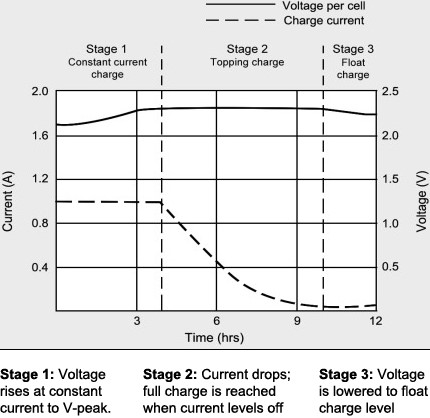
\includegraphics[scale=0.4]{Figures/cc.jpg}
\caption{Charging states of lead acid battery \cite{RS}}
\label{fig:states}
\end{wrapfigure}
 Battery charging tends to take on three different stages, these three stages can be referred to as bulk, absorption and float\cite{CC}.In the bulk charging stage the current is held at a constant amount and the voltage increases. For our battery this means 0.2-0.3C until the voltage reaches 6.75V\cite{RS}. The bulk stage includes the highest charging rate. During the absorption stage the voltage remains constant and the current decreases which leads to a decreasing charge rate. For our battery this means 0.1C until the voltage reaches 7.2V\cite{RS}. At the the end of the absorption stage the battery is at 100\% capacity. The next stage of charging is float charging where the voltage is decreased slightly (in our case to 6.75 - 6.9) and the current is at approximately 1\% of the battery capacity, this charging state is used to keep the battery charged indefinitely \cite{CC}. All these different states can be seen in figure \ref{fig:states} 






\label{sec:Discharge}
\par The C rating is a measurement of the rate at which a battery will discharge relative to its maximum capacity\cite{MIT}. 
\begin{wrapfigure}{l}{0.57\textwidth}
\centering
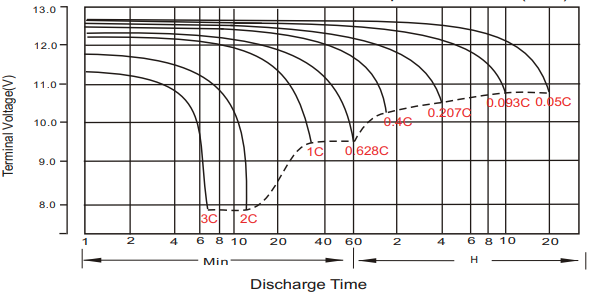
\includegraphics[scale=0.5]{Figures/fig2.png}
\caption{Discharge Characteristics \cite{Charging-Lead}}
\label{fig:discharge}
\end{wrapfigure}
 As the C rating decreases the run time does not increase linearly (refer to figure \ref{fig:discharge}), the reason for this is because a higher discharge rate causes the battery to lose energy to heat as more current flows through the internal resistance \cite{pSonic}. At higher discharge rates the terminal voltage is lower due to the internal resistance causes a voltage drop.


%%%%%%%%%%%%%%%%%%%%%%%%%%%%%%%%%%%%%%%%%%%%%%%%%%%%%%%%%%%%%%%%%%%%%%

\section{Fuse Characteristics}\label{sec:fuse_lit}
In this section, the different characteristics of the blade fuse that is being used is discussed. A fuse has a \textbf{current rating} which refers to the nominal current that the fuse can handle although it is recommended that the current at an ambient temperature of 25\textdegree C not be higher than 75\% of this value \cite{LF}. Fuses operate by blowing when current higher than the nominal rated current flow through the fuse. For this reason when the ambient temperature increases, the current required to reach a point where the fuse will melt is lower than it would be for lower ambient temperatures. This can be seen in figure \ref{subfig:temp} line "B". Current and time have an inverse relationship as can be seen in figure \ref{subfig:c-t}, this means that for higher currents the fuse will blow faster.


 \begin{figure}[!htb]
 \footnotesize
 \centering
    \begin{subfigure}[]{0.42\textwidth}
              \centering
  		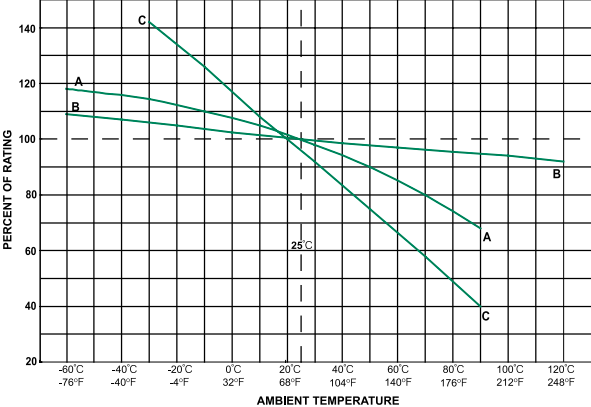
\includegraphics[width=1\linewidth]{./Figures/temperature.png}
		    \caption{} \label{subfig:temp}
     \end{subfigure}
     \begin{subfigure}[]{0.3\textwidth}
             \centering
  		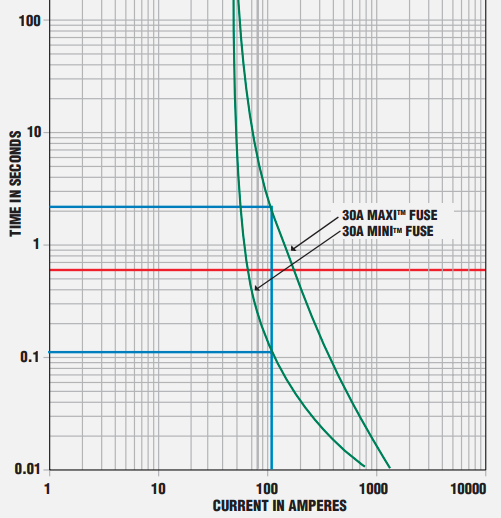
\includegraphics[width=1\linewidth]{./Figures/c-t.png}
		   \caption{ } \label{subfig:c-t}
     \end{subfigure}
   \caption[{Fuse Characteristics}]{Fuse Characteristics Relating to blow time   (a)  Current Rating versus Ambient Temperature\cite{LF} (b)  Blow time vs Current \cite{LF2} }
    \label{fig:two}
 \end{figure}


